\documentclass[11pt]{article}
\setlength{\textwidth}{7in}
\setlength{\topmargin}{-.5in}
\setlength{\textheight}{9in}
\setlength{\oddsidemargin}{-.25in}
\setlength{\evensidemargin}{-.25in}

\usepackage[noend]{algpseudocode}
\usepackage[]{fancyhdr}
\usepackage{amsmath}
\usepackage{hyperref}
\usepackage{cleveref}
\usepackage{graphicx}  % Required for inserting images
\usepackage{float} 

% Define title, author, and date
\title{Installation of Nordic SDK(Zephyr RTOS)}
\author{Jaehah Shin}  % Add author name here
\date{\today}         % You can replace \today with a custom date if needed

\begin{document}
\setlength{\headheight}{15.2pt}
\fancyhead{}
\pagestyle{fancy}

% Generate title block
\maketitle

% Your content here



\section{Introduction}
In this document, we will go through the installation of Nordic SDK. The installation of this SDK is essential for developing applications for the nRF52 series of microcontrollers. As we are going to use the nRF52840 chip for our final prototype, we need to install these SDKs to develop applications. First of all, this is important to know what zephyr and nordic SDKs are.
Zephyr RTOS is "The Zephyr OS is based on a small-footprint kernel designed for use on resource-constrained and embedded systems: from simple embedded environmental sensors and LED wearables to sophisticated embedded controllers, smart watches, and IoT wireless applications." \url{https://docs.zephyrproject.org/latest/introduction/index.html} In short, Zephyr RTOS is a real time operating system for embedded systems like macos or windows for computers. If you would like to know more about Zephyr RTOS, please visit the link above. Nordic SDK is a software development kit for nRF52 series of microcontrollers. It provides libraries and examples for developing applications for nRF52 series of microcontrollers.
Also, nordic SDK is based on Zephyr RTOS and Zephyr RTOS is integrated into Nordic SDK. Therefore, installing Nordic SDK will also install Zephyr RTOS in their SDK.

\section{Installation of Nordic SDK}
\subsection{installations}
There are in total 3 installations that we need to do for developing applications for nRF52 series of microcontrollers. \\
1. Install nRF Command Line Tools \\
2. Install nRF Connect for Desktop \\
3. Install nRF Connect in Visual Studio Code \\
There are three different operating system depends on what you are running on your computer. This is supported on \textit{Windows, MacOS, and Linux} operating systems.
As general steps are identical for all three operating systems (I have tested on Windows 11 home, pro, MacOS silcon, and Ubuntu), you can just follow the steps below. \\
Please note that you should know what operating system you are running on your computer. \\
\subsection{Install nRF Command Line Tools}
This tool is essential for development, programming and debugging with nRF52 series of microcontrollers. \\
To install this, please visit the link below and download the installer for windows. \\
\url{https://www.nordicsemi.com/Products/Development-tools/nRF-Command-Line-Tools}

\begin{figure}[H]
\centering
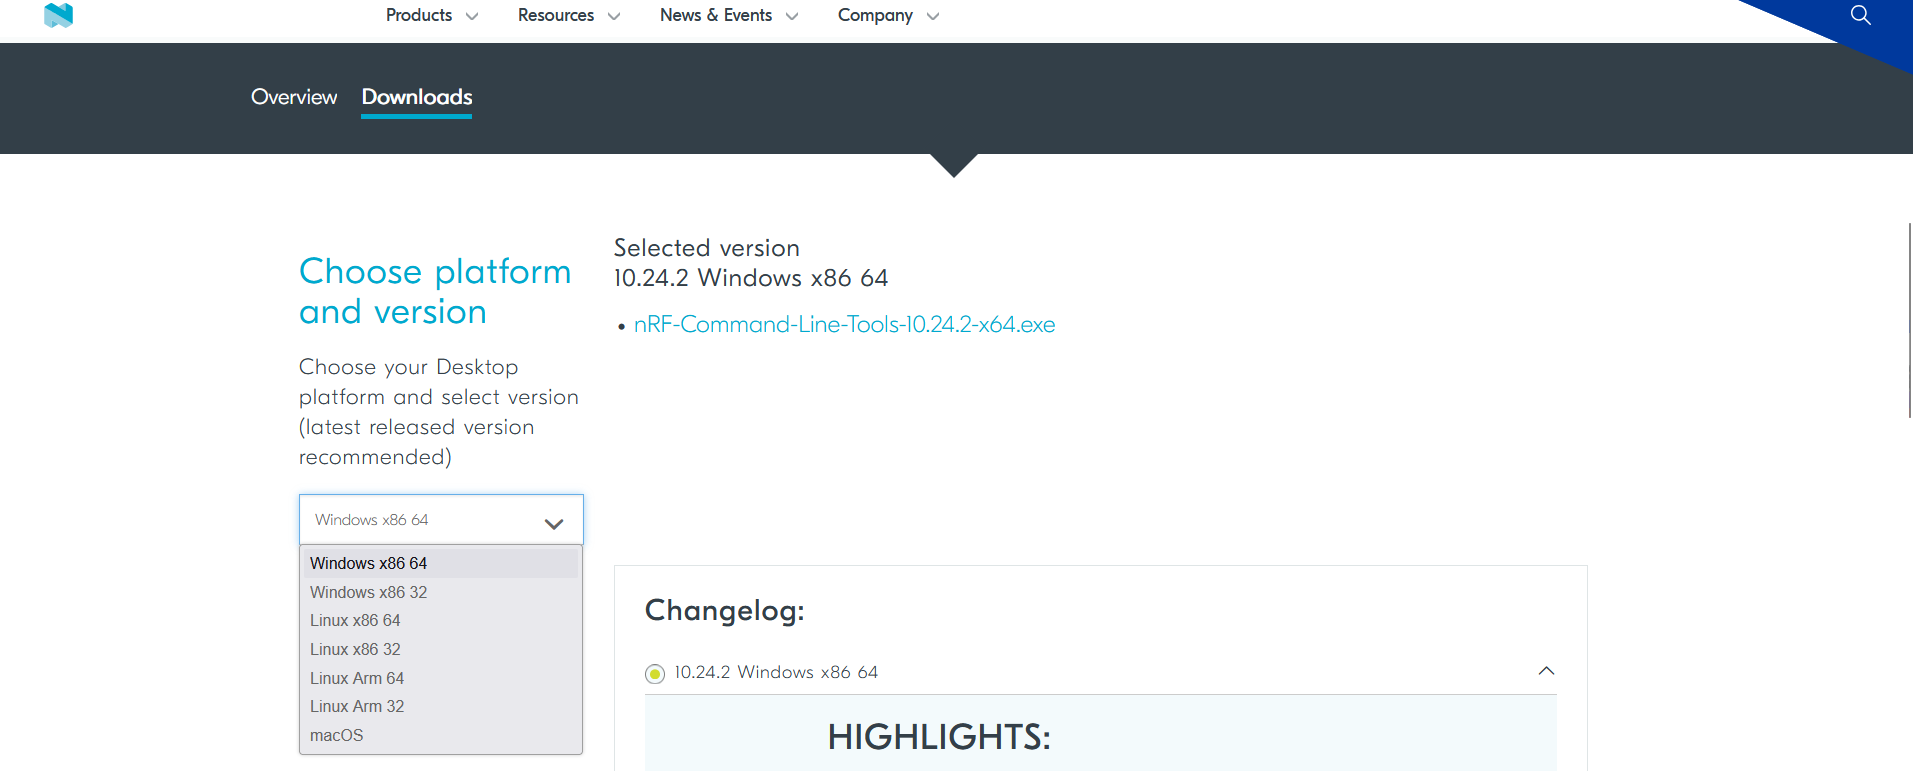
\includegraphics[width=0.8\textwidth]{command.png}
\caption{Nordic Commandline Tools Download Page}
\label{fig:command_line_tools}
\end{figure}
As you can see from dropdown menu, you can select the operating system you are running on your computer. 
Also, you can see the version of the installer, and I would recommend you to download the latest version of the installer. (nRF-Command-Line-Tools-10.24.2-x64.exe as 2024/09/30) \\
Usually, you can click the blue link to download the latest version of the installer. \\

\subsection{Install nRF Connect for Desktop}
nRF Connect for Desktop is a cross-platform tool for developing nRF devices. It offers apps to test, monitor, measure, optimize, and program applications. Compatible with development kits and dongles, it detects connected kits and uploads the necessary firmware. Supported kits are listed in the documentation. \\
To install this, please visit the link below and download the installer for windows. \\
\url{https://www.nordicsemi.com/Products/Development-tools/nRF-Connect-for-Desktop}

\begin{figure}[H]
    \centering
    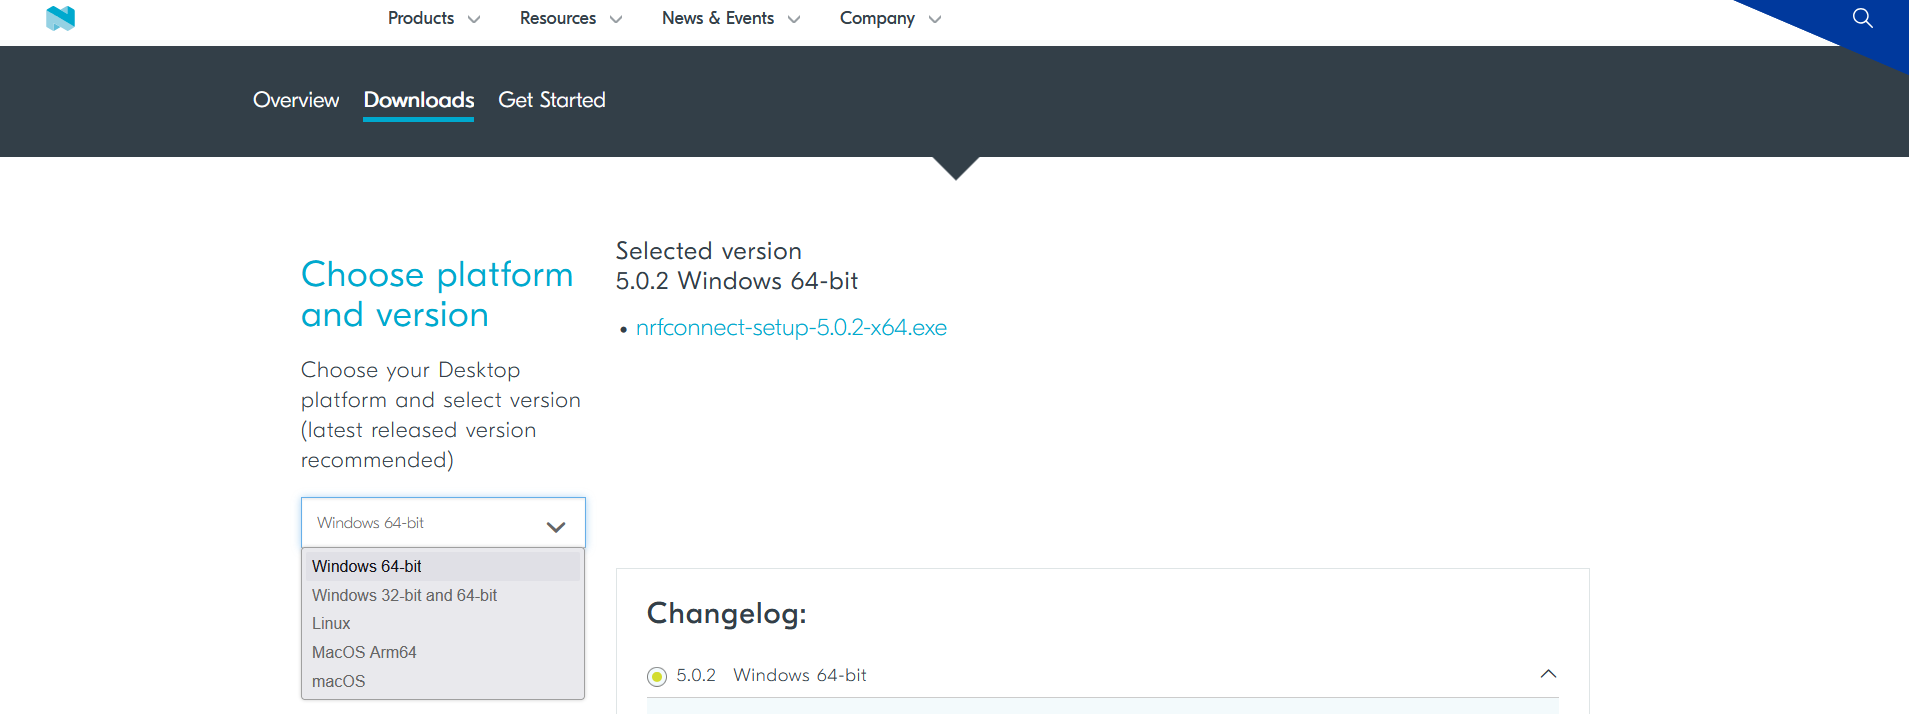
\includegraphics[width=0.8\textwidth]{sdk.png}
    \caption{nRF Connect for Desktop Download Page}
    \label{fig:command_line_tools}
    \end{figure}
Here is the same. You can select the operating system you are running on your computer. Also, be sure to download the latest version of the installer. (Blue linked text) \\

\subsection{Install nRF Connect in Visual Studio Code}
This is an extension for Visual Studio Code. With this you can look at devicetree, build, flash and debug applications for nRF52 series of microcontrollers. \\
To install this, please go to extension tab in Visual Studio Code and search for nRF Connect for VScode. Then install the extension. \\

\begin{figure}[H]
    \centering
    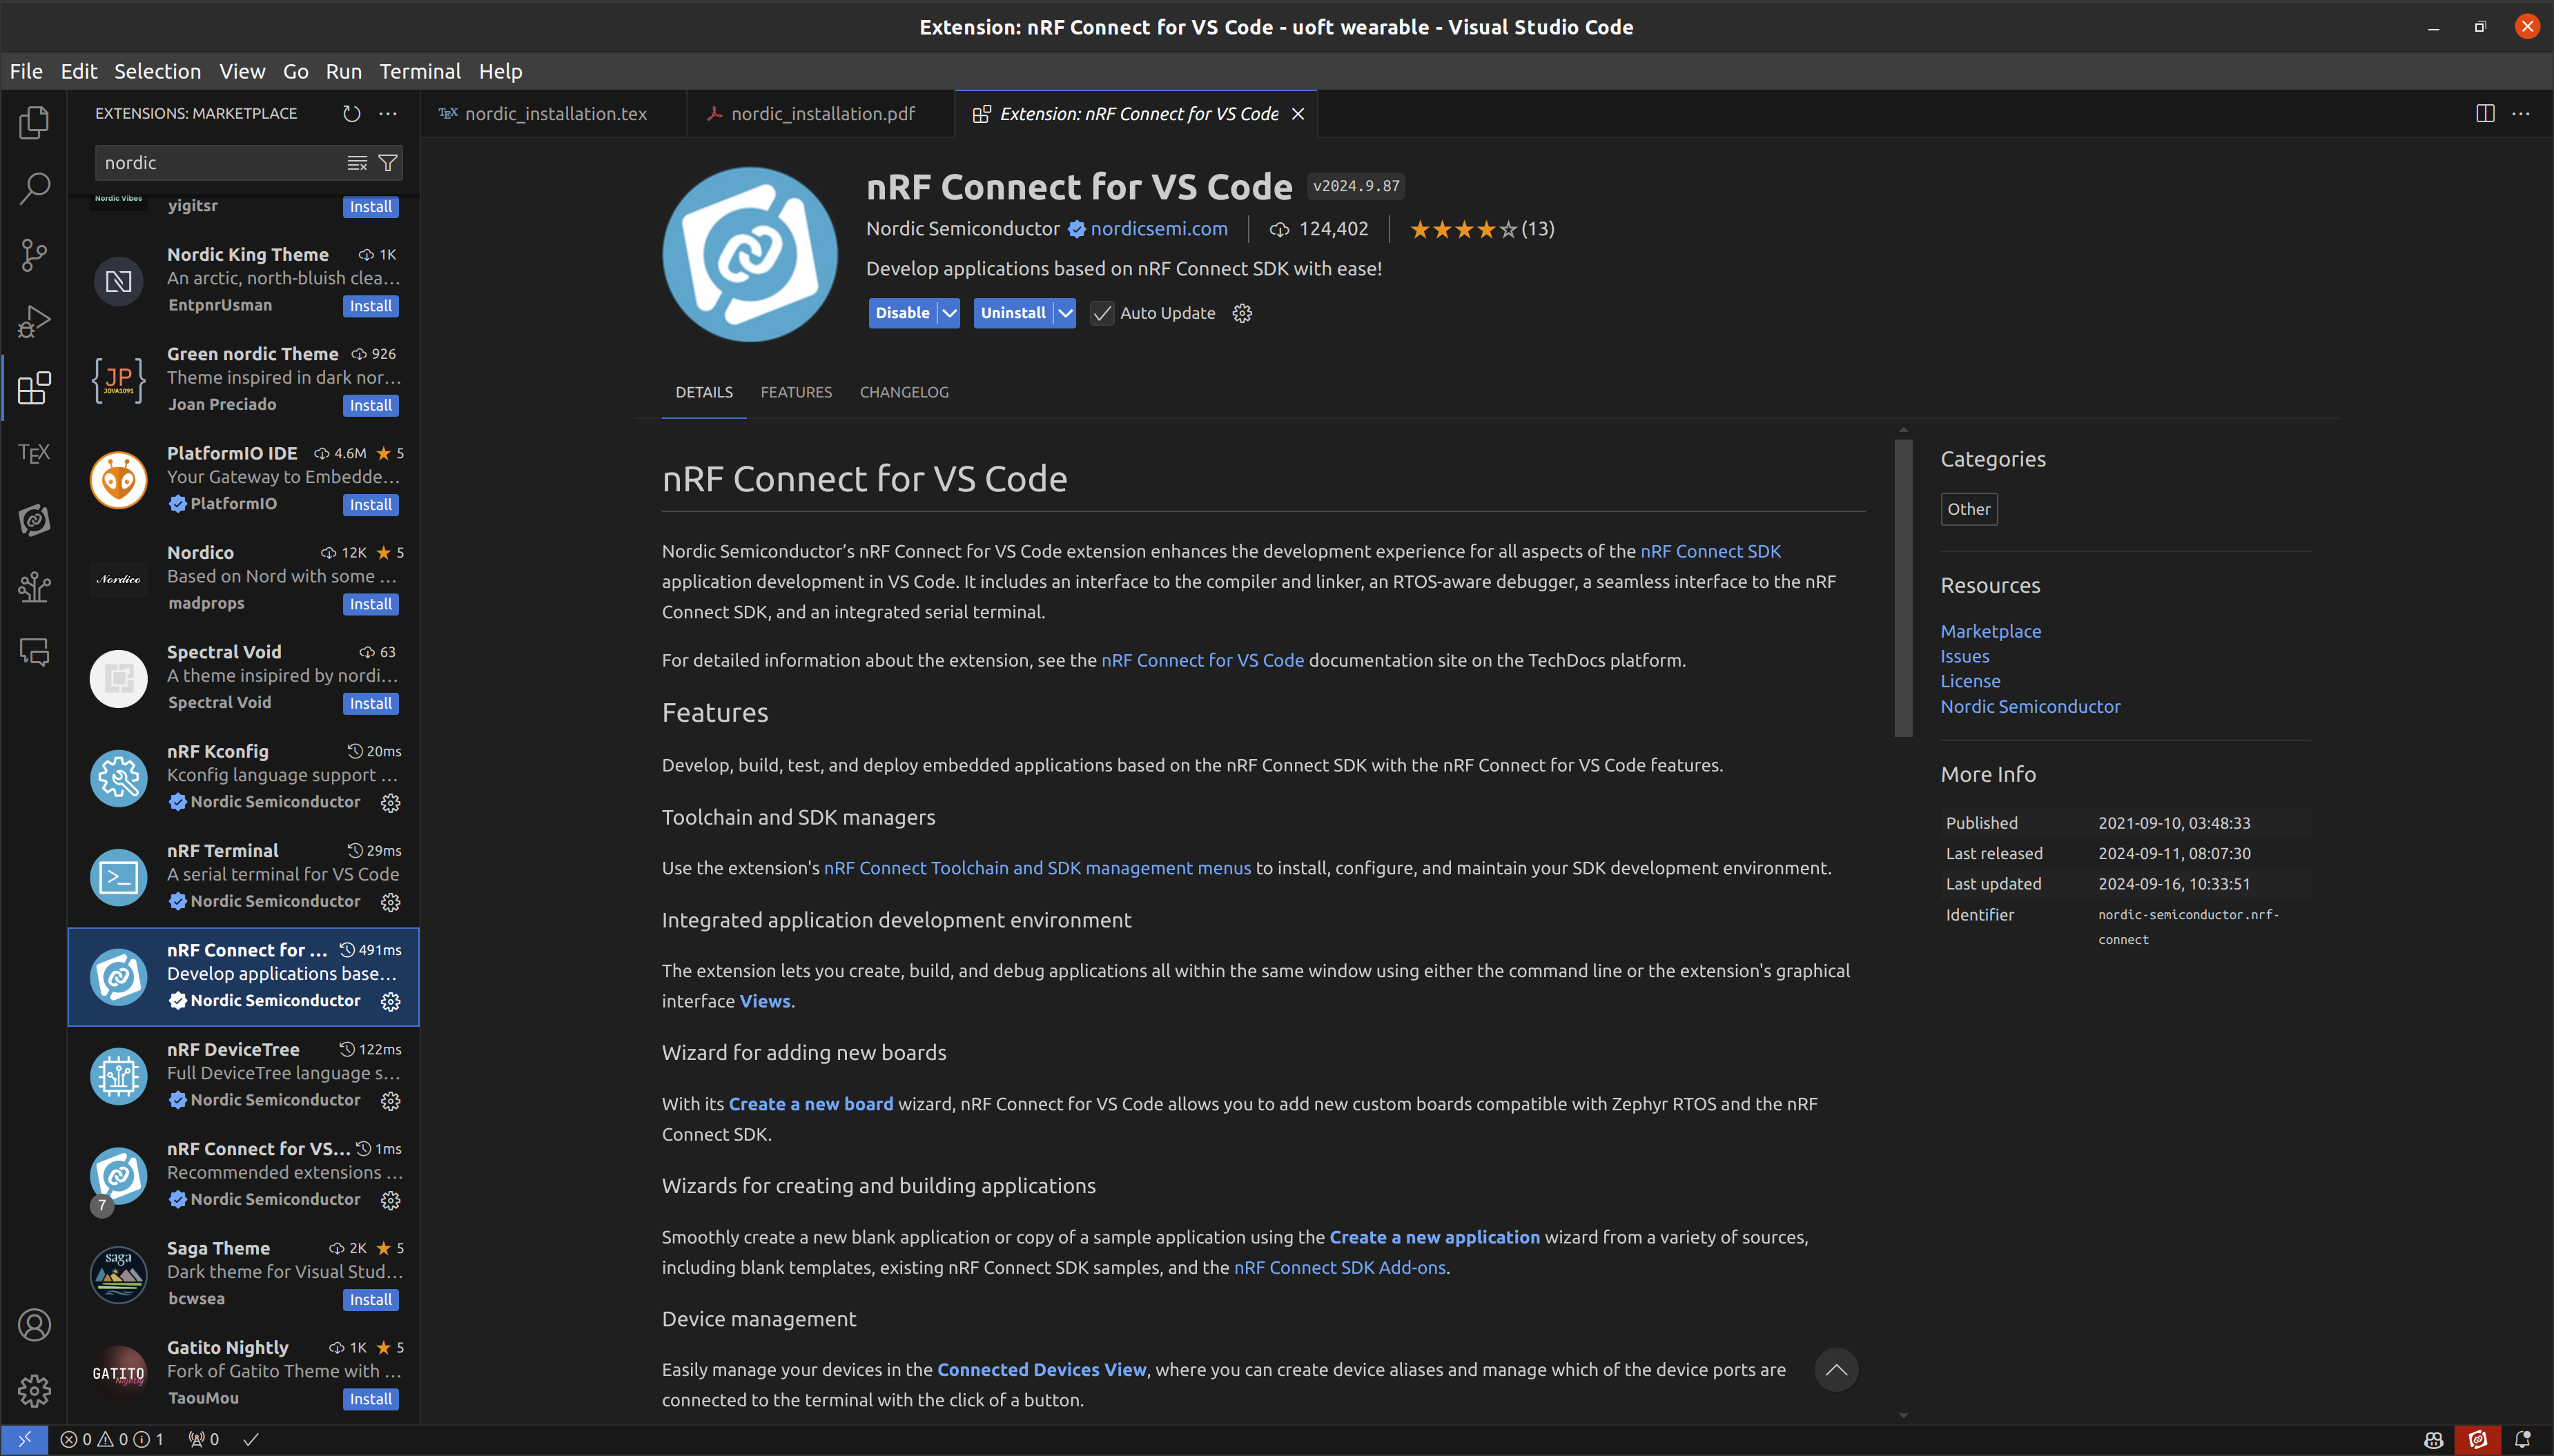
\includegraphics[width=0.8\textwidth]{github.png}
    \caption{nRF Extension in Visual Studio Code}
    \label{fig: Extension in Visual Studio Code}
    \end{figure}

You can select the extension in the figure \ref{fig: Extension in Visual Studio Code} and click install button. \\   
\section{Next Steps}
After you complete the installations, there is one more step you need to do. \\
You need to open the nRF Connect for Desktop and you will see this page. 

\begin{figure}[H]
    \centering
    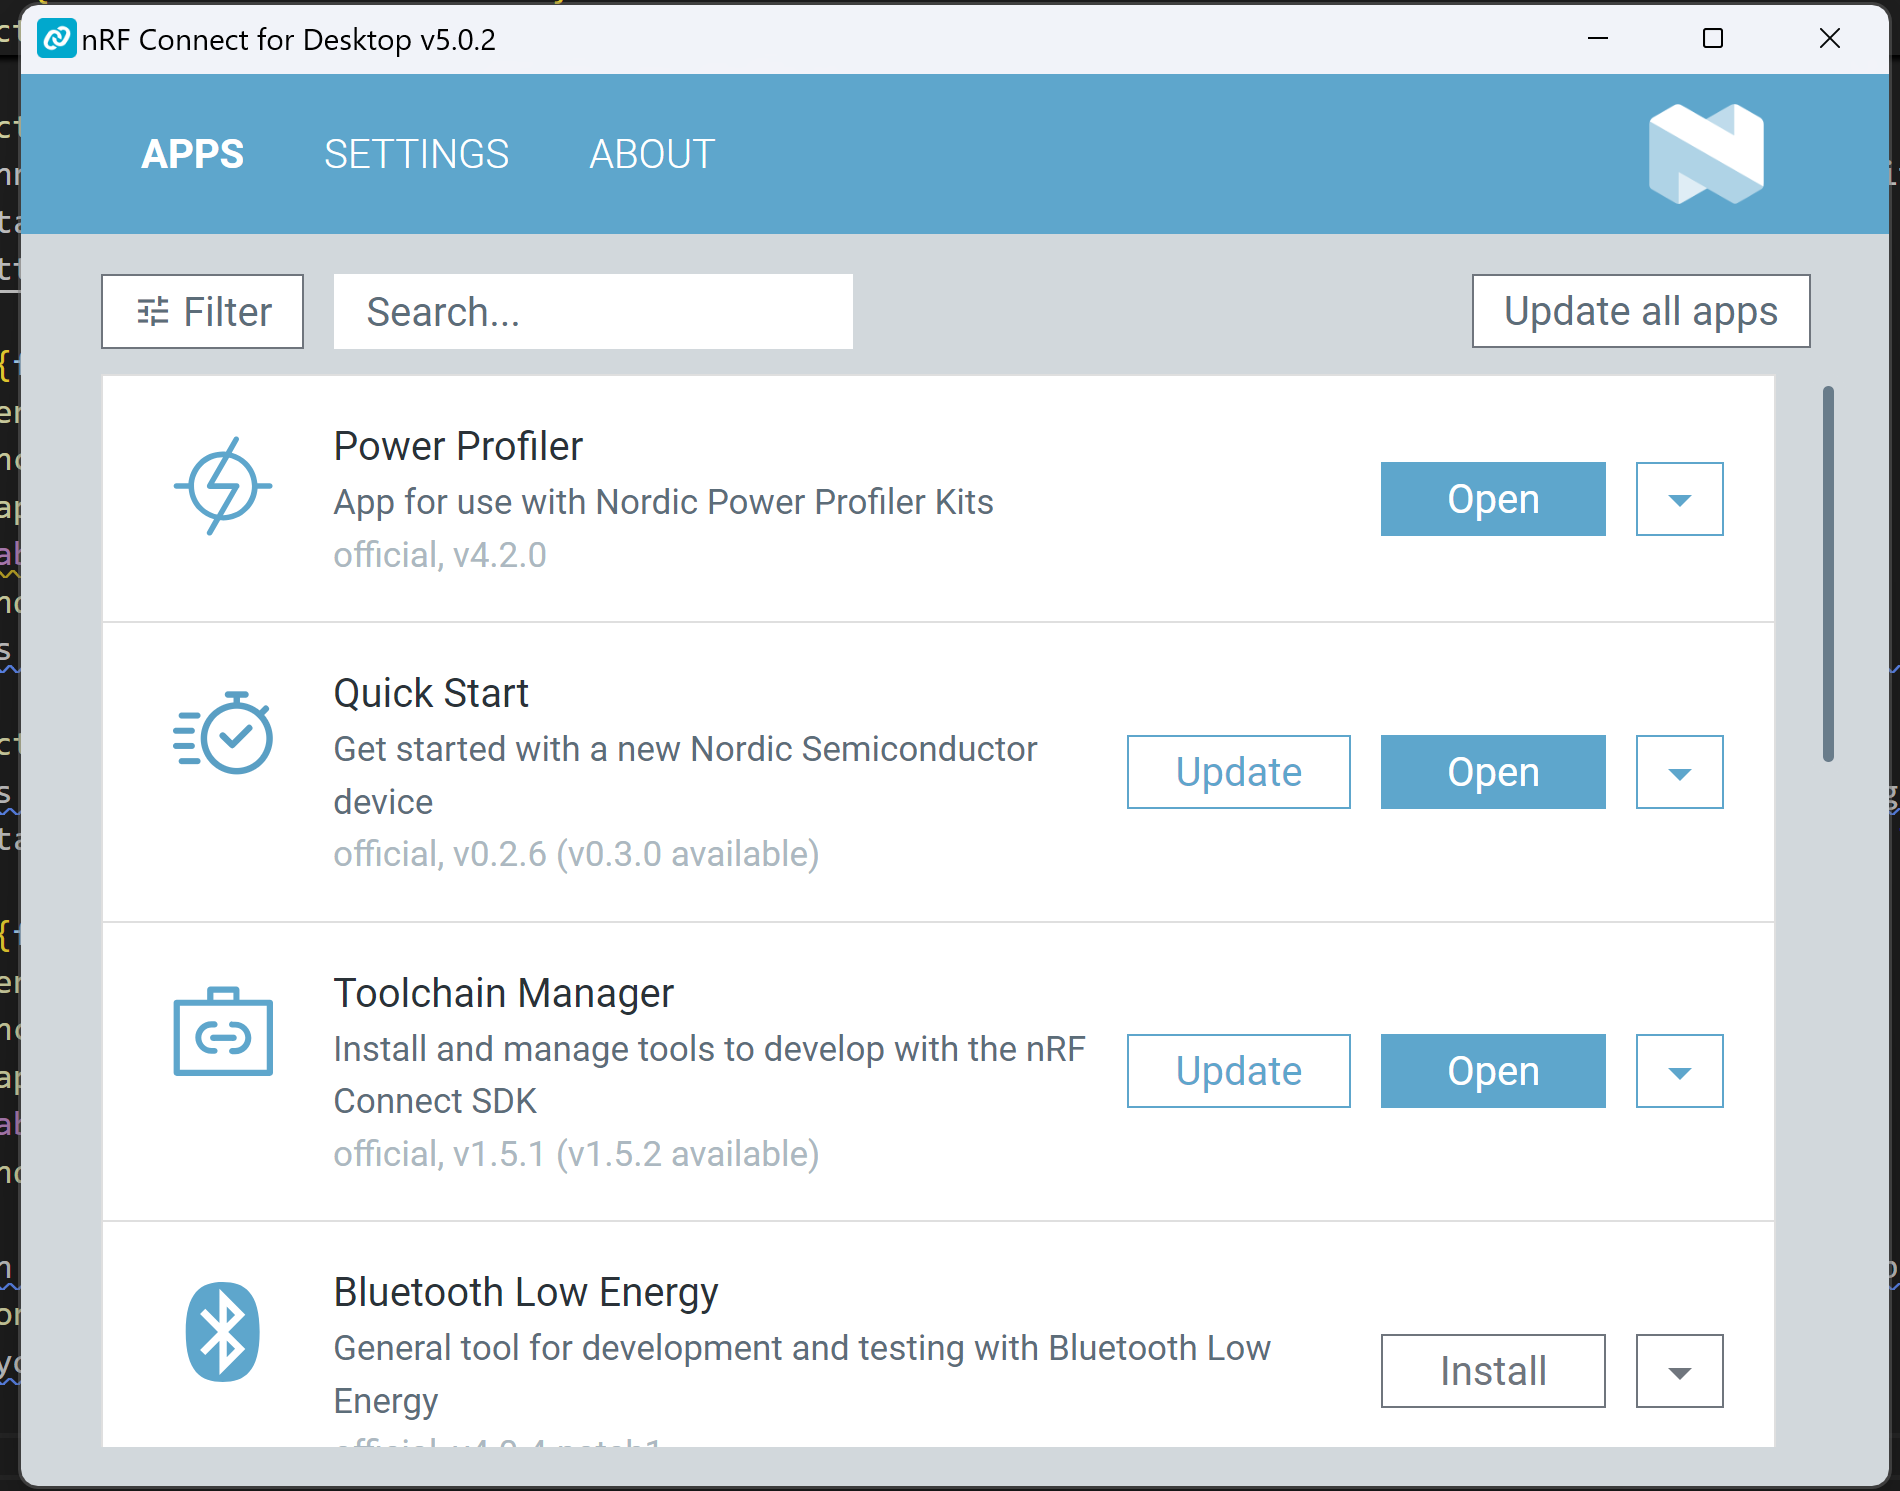
\includegraphics[width=0.6\textwidth]{nrf.png}
    \caption{nRF Connect for Desktop}
    \label{fig: nRF Connect for Desktop}
    \end{figure}
You will now have to click the \textit{install} button for toolchain manager to install the toolchain. \\
After installing the toolchain, open the toolchain manager. You will see the page below.

\begin{figure}[H]
    \centering
    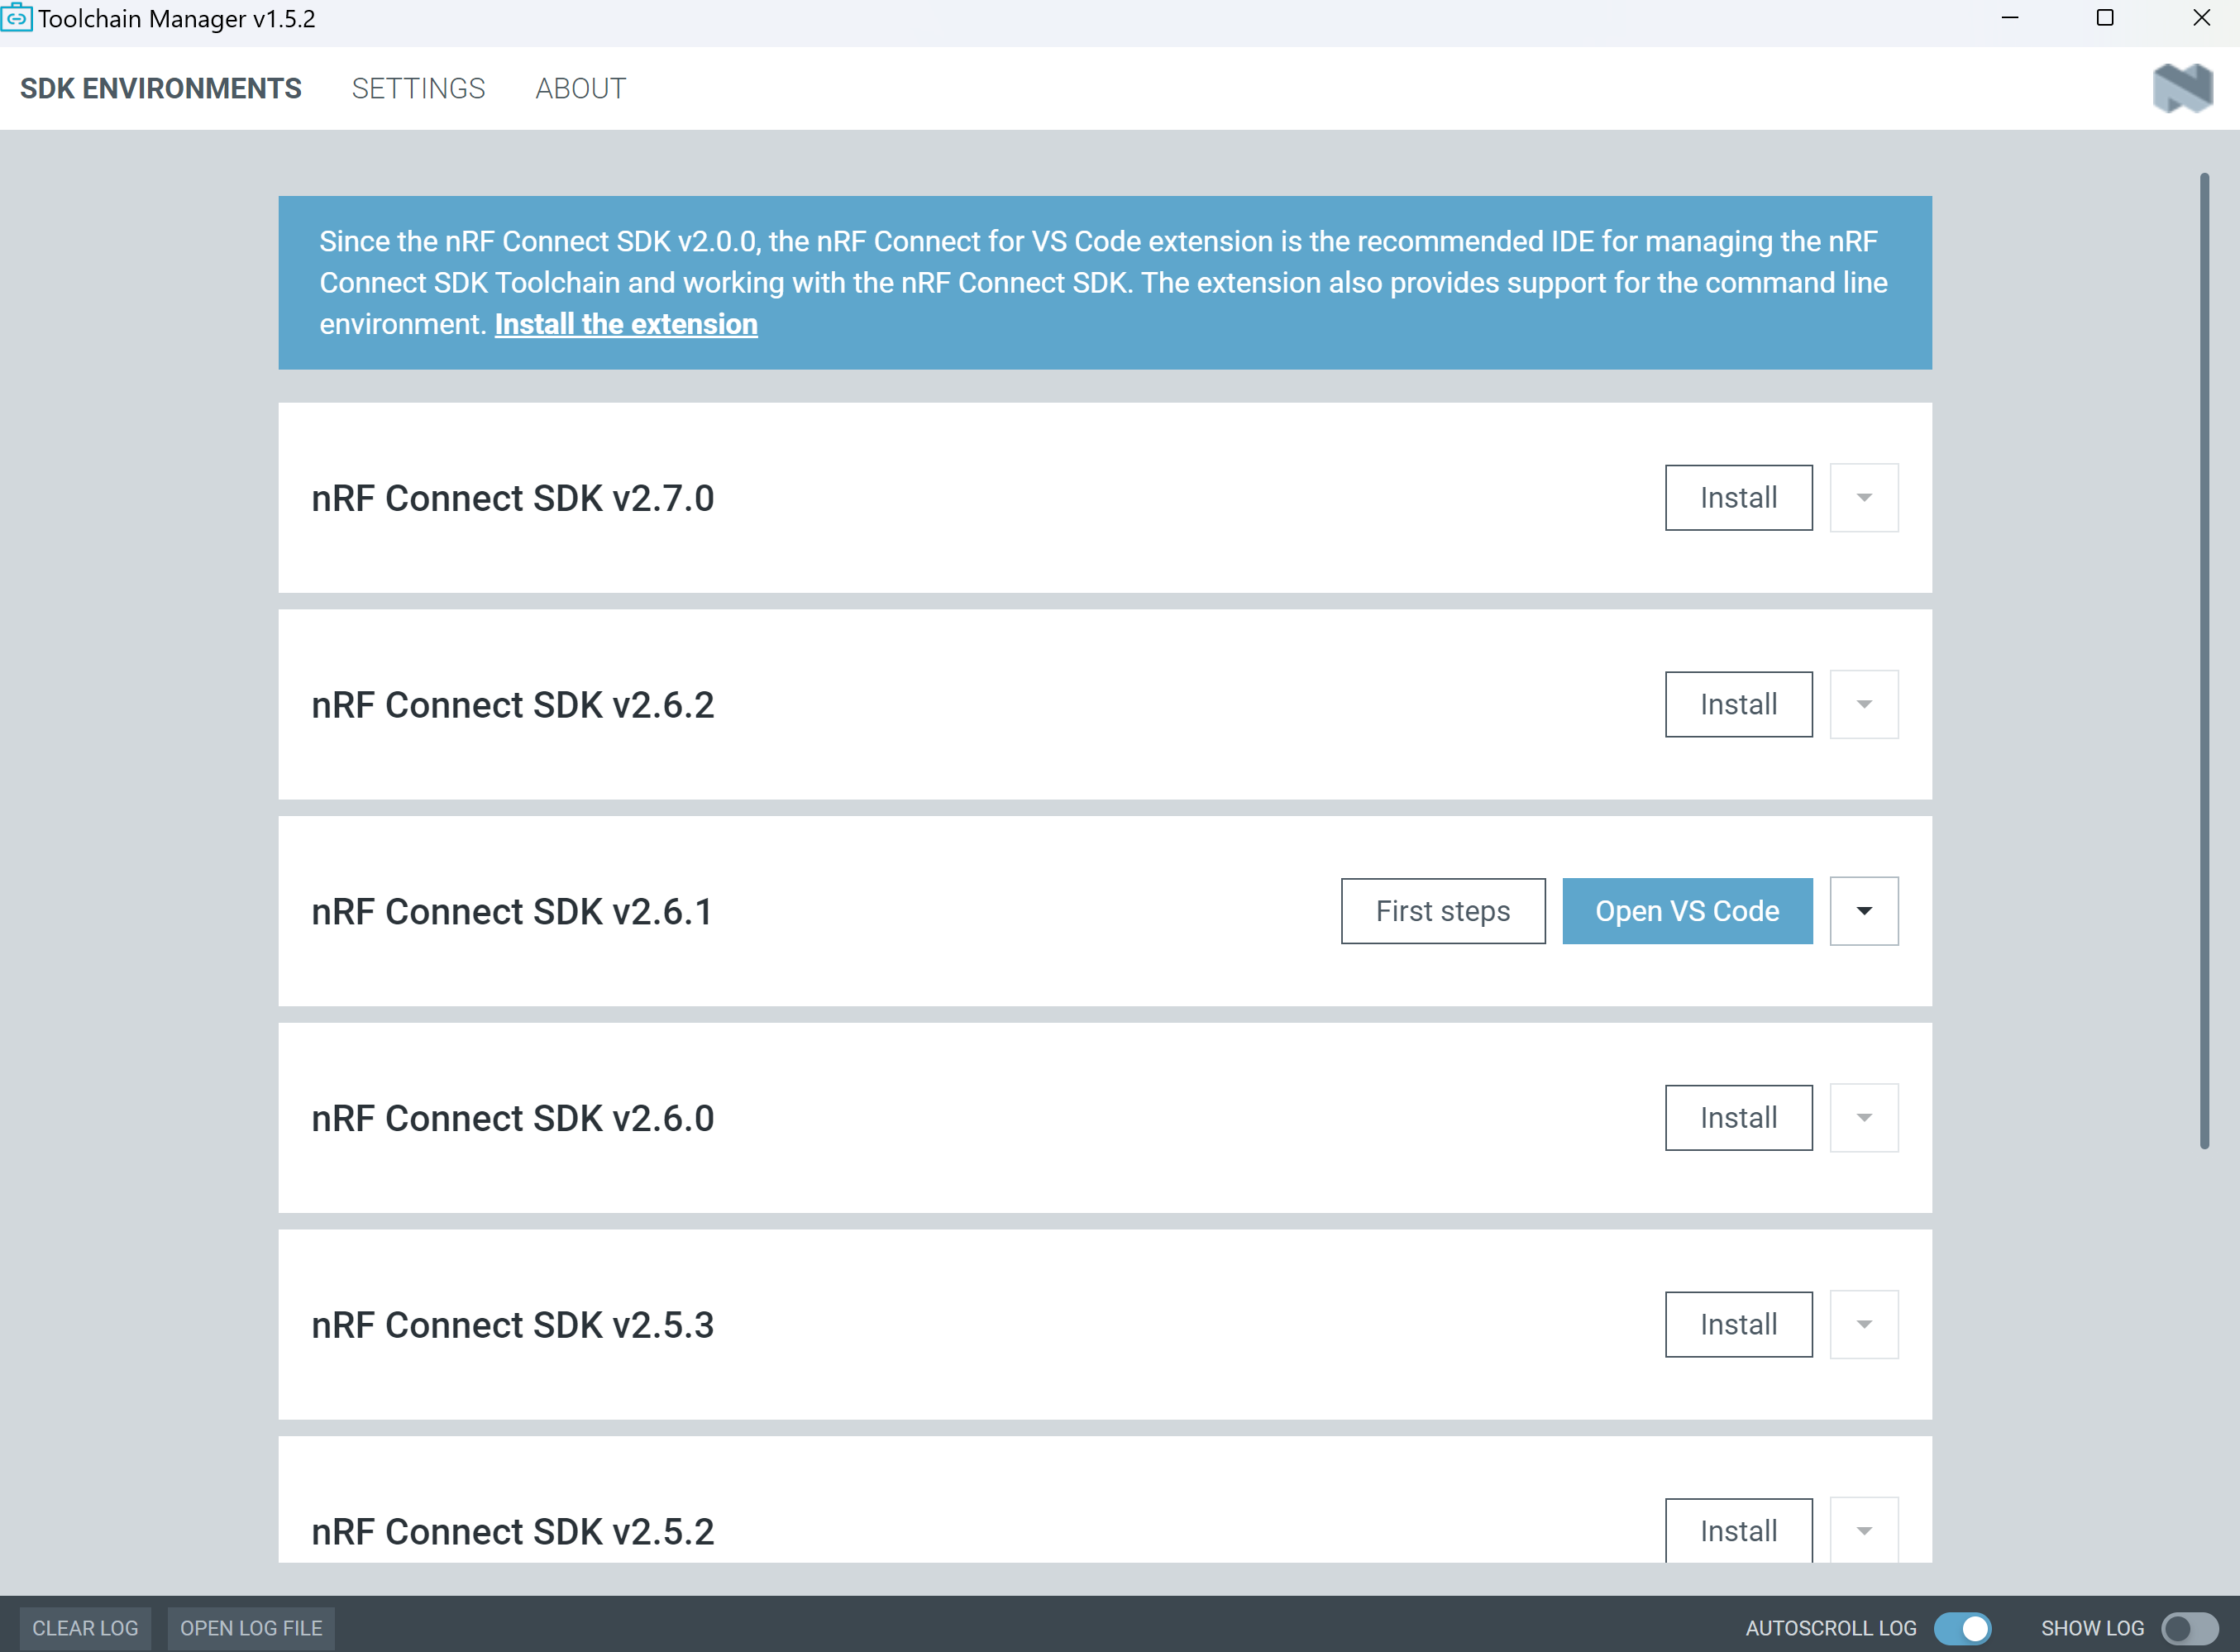
\includegraphics[width=0.6\textwidth]{toolchain.png}
    \caption{Toolchain Manager}
    \label{fig: Toolchain Manager}
    \end{figure}
Now, I recommend you to install the latest version of the toolchain whenever you are completing this tutorial. \\

\section{Conclusion}
In this document, we have gone through the installation of Nordic SDK. This is essential for developing applications for nRF52 series of microcontrollers. We have installed nRF Command Line Tools, nRF Connect for Desktop, and nRF Connect in Visual Studio Code. Also, we have installed the toolchain for developing applications. 
Well done! You have completed the installation of Nordic SDK. Now you are ready to develop applications for nRF52 series of microcontrollers. \\
If you have any questions, please feel free to ask me. \\












\end{document}
